
%--------------------------------------------------------------------
\section{Anomaly Detection}
%--------------------------------------------------------------------

\ifnum\short=0

\begin{frame}
    \frametitle{Suspicious Behavior Detection from a Small Bootstrap Set}
    \framesubtitle{Introduction}

    Automatic anomaly detection can improve video surveillance systems. 
    State-of-the-art methods look for unusual changes in the global 
    foreground mask. Research on local behavior modeling for predefined 
    behaviors is mature.

    \bigskip 

    We explore a new and effective algorithm for semi-supervised learning 
    of common human behaviors and detect anomalies in video sequences.
  
\end{frame}

%--------------------------------------------------------------------

\begin{frame}
    \frametitle{Suspicious Behavior Detection from a Small Bootstrap Set}
    \framesubtitle{Related Work}

    Some of the existing work relies on having a priori known behavior
    classes (Nair and Clark, 2002; Wu et al., 2005).

    \bigskip

    Other work (Lee et al., 2003; Wu et al., 2005; Arsi{\'c} et al., 2007)
    uses support vector machines (SVMs) to model and classify behaviors 
    into pre-defined classes.

\end{frame}

%--------------------------------------------------------------------

\begin{frame}
    \frametitle{Suspicious Behavior Detection from a Small Bootstrap Set}
    \framesubtitle{Related Work (cont.)}

    There has been some work on anomalous time series detection 
    outside the context of video surveillance using relatively 
    simple statistical models (Turner et al., 2010; Yao et al., 2010).

    \bigskip

    However, these methods learn single comprehensive models 
    without addressing the special requirement in video 
    surveillance to capture an extremely wide variety of typical 
    behaviors. This requires construction of a collection of 
    statistical models.

    \bigskip 

    Intrusion detection requires similar diversity in the 
    statistical models.

\end{frame}

%--------------------------------------------------------------------

\begin{frame}
    \frametitle{Detection from a Small Bootstrap Set}
    \framesubtitle{Methodology}

    \begin{itemize}
        \item Blob extraction and tracking from ``Blob-Based Motion Anlaysis''
        \item Behavior model bootstrapping from ``Clustering Human Behaviors''
        \item Anomaly Detection
    \end{itemize}

\end{frame}

%--------------------------------------------------------------------

\begin{frame}
    \frametitle{Detection from a Small Bootstrap Set}
    \framesubtitle{Anomaly Detection}

    \begin{itemize}
        \item Pure supervised approach is obviously not suitable, however, 
            when examples of anomalous behavior are sparse or nonexistent.
        \item Unsupervised approach has the difficulty that there is no clear 
            way to calibrate the parameters of the ``too far'' cirterion.
        \item We propose a {\em semi-supervised} approach that self-calibrates 
            itself from a small bootstrap set in which each bootstrap sequence 
            is manually labeled as normal or suspisous by a human operator.
    \end{itemize}

\end{frame}

%--------------------------------------------------------------------

\begin{frame}
    \frametitle{Detection from a Small Bootstrap Set}
    \framesubtitle{Pseudocode for Anomaly Detection}

    \begin{algorithm}[H]
        \caption{Anomaly Detection}
        \begin{algorithmic}
            \REQUIRE $\vec{O}$: behavior sequence
            \REQUIRE ${\cal M}$: set of HMMs
            \STATE ${\cal M}_{ab} \gets \{ M \mid M \in {\cal M} \text{~and $M$ is marked abnormal} \}$
            \STATE $( M_{ml}, L_{ml} ) \gets \textsc{Find-Most-Likely-Model}(\vec{O}, {\cal M})$
            \IF{$M_{ml} \in {\cal M}_{ab}$ or $L_{ml} \leq \theta_z$}
                \STATE $\textsc{Alert-Security-Personnel}(\vec{O})$
            \ENDIF
        \end{algorithmic}
    \end{algorithm}

\end{frame}

%--------------------------------------------------------------------

\begin{frame}
    \frametitle{Detection from a Small Bootstrap Set}
    \framesubtitle{Experimental Results}

    We select the model configuration with the highest accuracy in separating 
    the normal sequences from the abnormal sequences on the boostrap set, as 
    measured by the false positive rate for abnormal sequences.
    \begin{figure}
        \centering
        \begin{tabular}{ccc}
            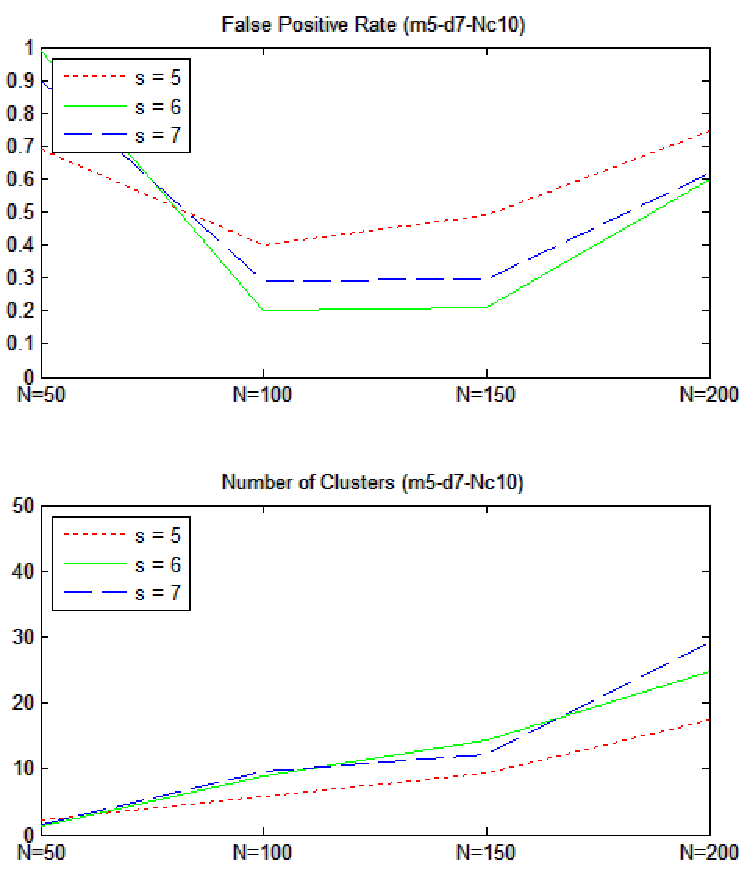
\includegraphics[scale=0.23]{figures/model-configuration01} &
            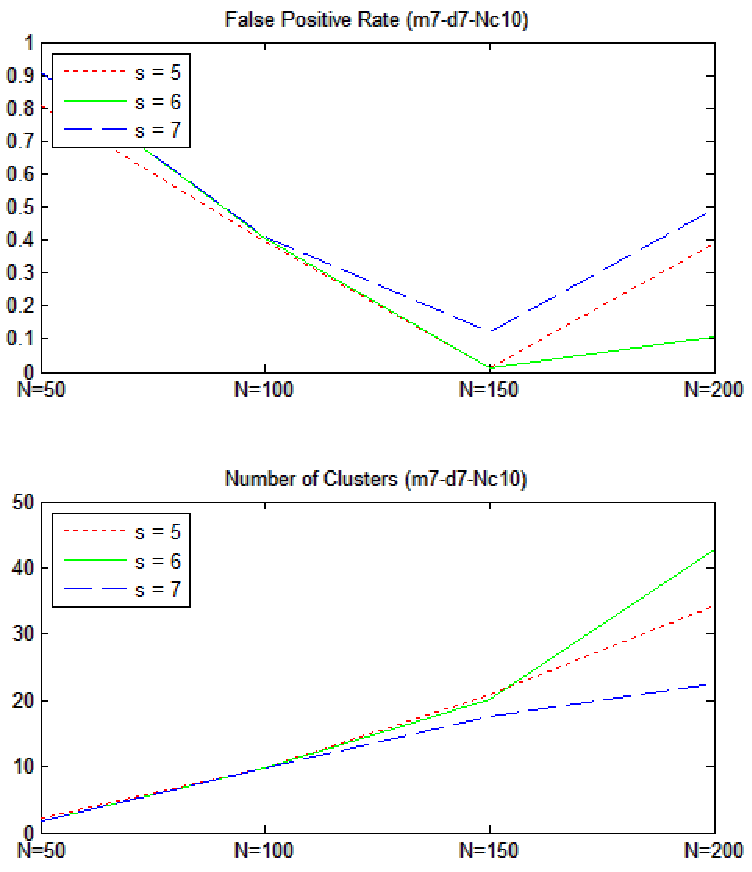
\includegraphics[scale=0.23]{figures/model-configuration02} &
            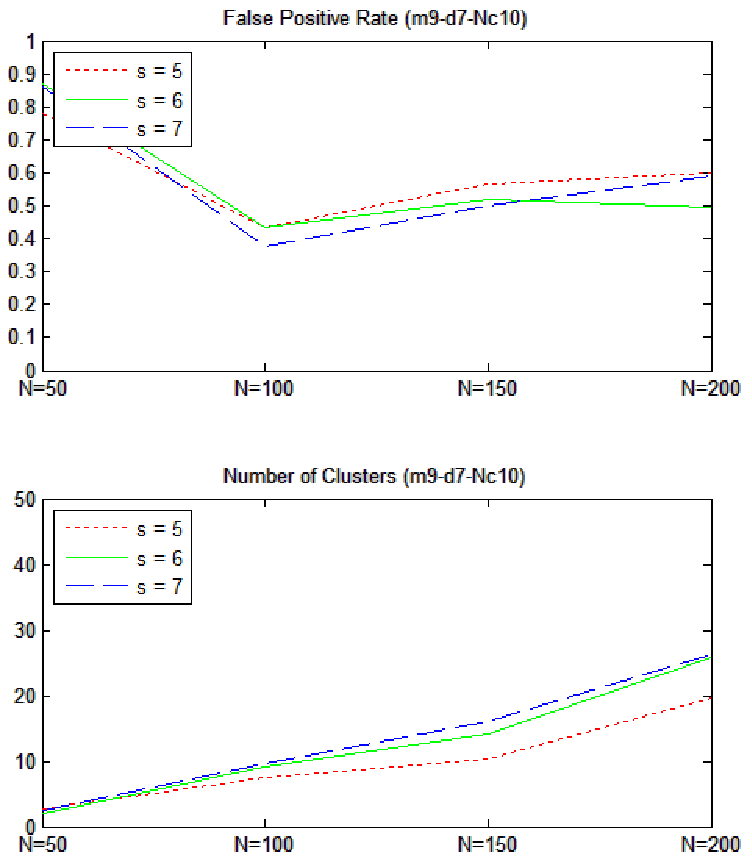
\includegraphics[scale=0.23]{figures/model-configuration03}\\
            (a) & (b) & (c)
        \end{tabular}
        \caption{Subset of model configuration selection results.  Model
            configuration with (a) five tokens, (b) seven tokens and (c) nine
            tokens. Red, green and blue lines represent models with five, six
            and seven states, respectively.  Each point is an average over 10
            trials.}
        \label{fig:batch-some-clustering-results}
    \end{figure}

\end{frame}

%--------------------------------------------------------------------

\begin{frame}
    \frametitle{Detection from a Small Bootstrap Set}
    \framesubtitle{Experimental Results (cont.)}

    \vspace{-0.1in}
    \begin{table}
        \caption{Example human behavior pattern bootstrapping
        results. We used linear HMMs with five states and seven
        tokens. The model consists of 20 clusters. ``W'' means ``walk''
        and ``C'' means ``cycle.''  For the seven clusters containing more
        than one sequence, shown is the distribution of the patterns in
        the cluster over the activities.  The last row shows the
        distribution of the 13 clusters containing only a single sequence
        over the activity categories.}
        \centering
        \begin{tabular}{c|c|c|c|c|c}
            \hline
            Cluster \# & W-in & W-out & C-in & C-out & Other \\
            \hline \hline
            1 & 44 & 0 & 20 & 0 & 0 \\ \hline
            2 & 0 & 37 & 0 & 19 & 0 \\ \hline
            3 & 0 & 0 & 2 & 0 & 0 \\ \hline
            4 & 0 & 0 & 3 & 0 & 0 \\ \hline
            5 & 0 & 0 & 0 & 4 & 0 \\ \hline
            6 & 0 & 0 & 0 & 0 & 6 \\ \hline
            7 & 0 & 0 & 0 & 0 & 2 \\ \hline
            One-seq clusters & 0 & 2 & 6 & 2 & 3 \\ \hline
        \end{tabular}
    \end{table}

\end{frame}

%--------------------------------------------------------------------

\begin{frame}
    \frametitle{Detection from a Small Bootstrap Set}
    \framesubtitle{Experimental Results (cont.)}

    \begin{figure}
        \centering
        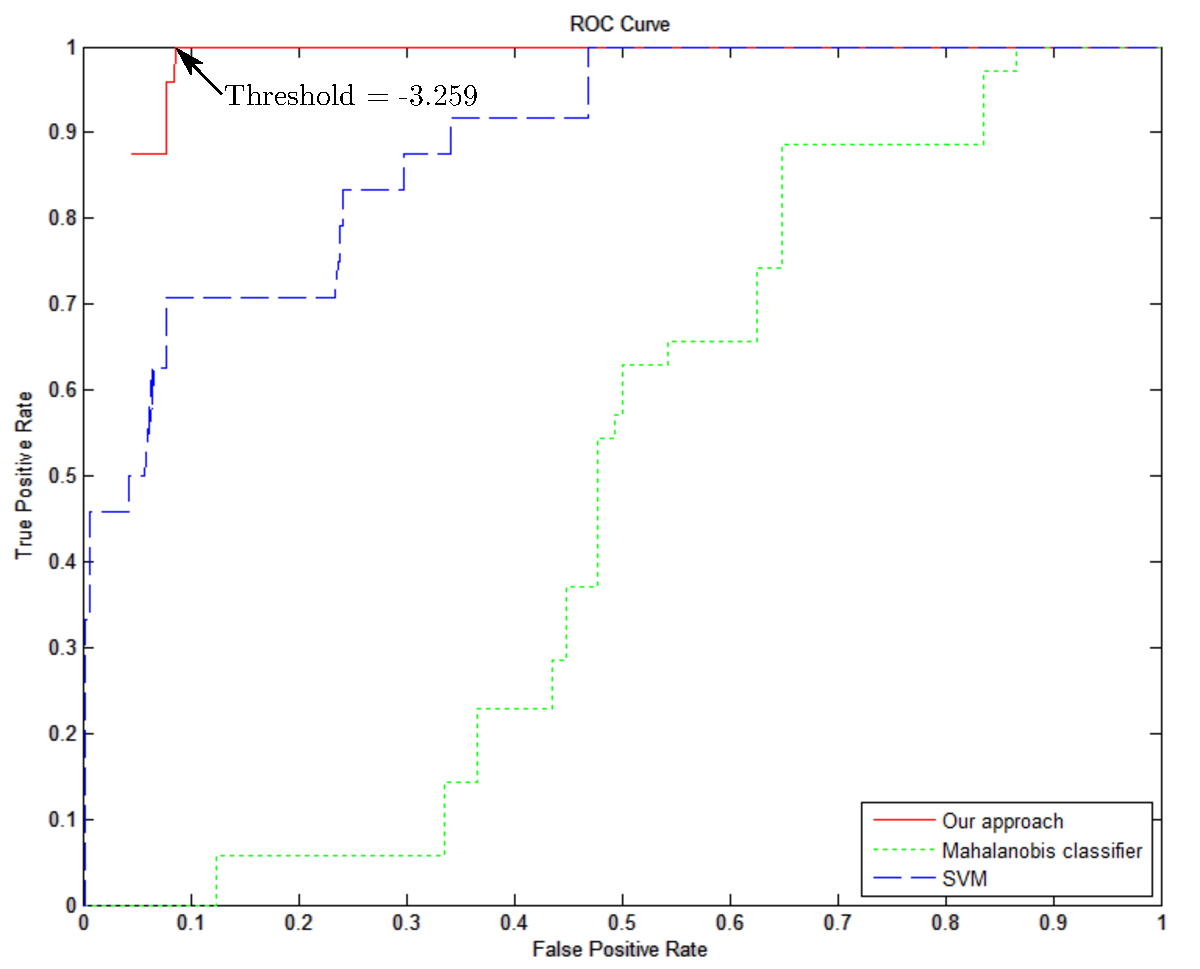
\includegraphics[width=0.5\linewidth]{figures/roc-ours-vs-ml-results}
        \caption{Anomaly
            detection ROC curves. Red, green, and blue lines represent ROCs
            for the proposed method, Mahalanobis classifier for anomaly 
            detection, and SVM-based anomaly detection, respectively.}
        \label{fig:batch-roc-results}
    \end{figure}

\end{frame}

%--------------------------------------------------------------------

\begin{frame}
    \frametitle{Detection from a Small Bootstrap Set}
    \framesubtitle{Experimental Results (cont.)}

    \begin{table}
        \caption{Anomaly detection results for the
            proposed method, $k$-NN anomaly detection method, Mahalanobis 
            classifier for anomaly detection method, and SVM-based anomaly 
            detection method, respectively. For the Mahalanobis classifier
            for anomaly detection method, we include 11 abnormal sequences from
            the bootstrap set in the test set, so the total number of
            positives is 35.}
        \centering
        \begin{tabular}{c|c|c|c|c|c|c}
            \hline
            Method & TP & FP & TN & FN & TPR & FPR \\
            \hline\hline
            Ours & 24 & 36 & 450 & 0 & 1 & 0.074 \\ \hline
            $1$-NN & 19 & 1 & 485 & 5 & 0.792 & 0.002 \\ \hline
            $2$-NN & 19 & 2 & 484 & 5 & 0.792 & 0.004 \\ \hline
            $3$-NN & 16 & 0 & 486 & 8 & 0.667 & 0 \\ \hline
            $4$-NN & 16 & 1 & 485 & 8 & 0.667 & 0.002 \\ \hline
            $5$-NN & 14 & 0 & 486 & 10 & 0.583 & 0 \\ \hline
            Mahalanobis classifier & 35 & 421 & 65 & 0 & 1 & 0.87 \\ \hline
            SVM & 24 & 228 & 258 & 0 & 1 & 0.469 \\ \hline
        \end{tabular}
        \label{tab:batch-detection-results}
    \end{table}

\end{frame}

%--------------------------------------------------------------------

\begin{frame}
    \frametitle{Detection from a Small Bootstrap Set}
    \framesubtitle{Experimental Results (cont.)}

    \begin{figure}[t]
        \centering
        \begin{tabular}{ccccc}
            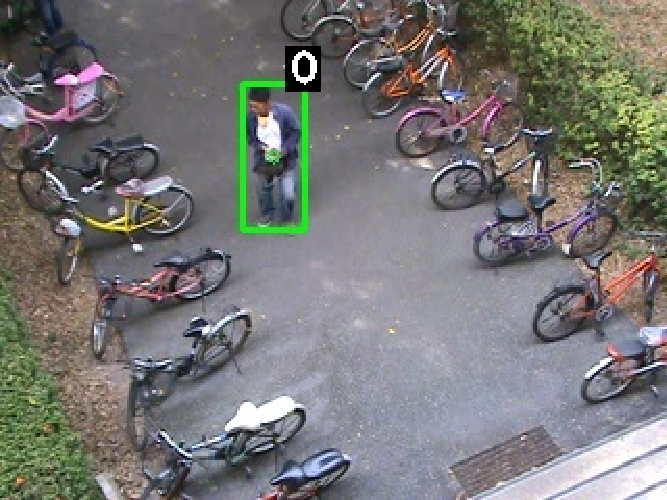
\includegraphics[scale=0.17]{figures/case-1-suspicious-0187} &
            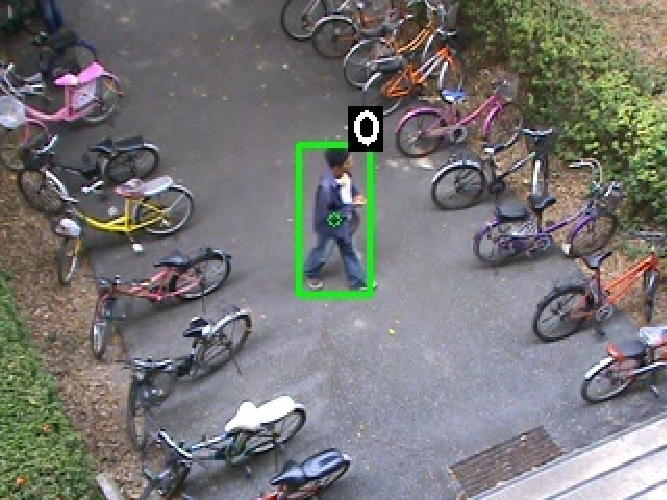
\includegraphics[scale=0.17]{figures/case-1-suspicious-0208} &
            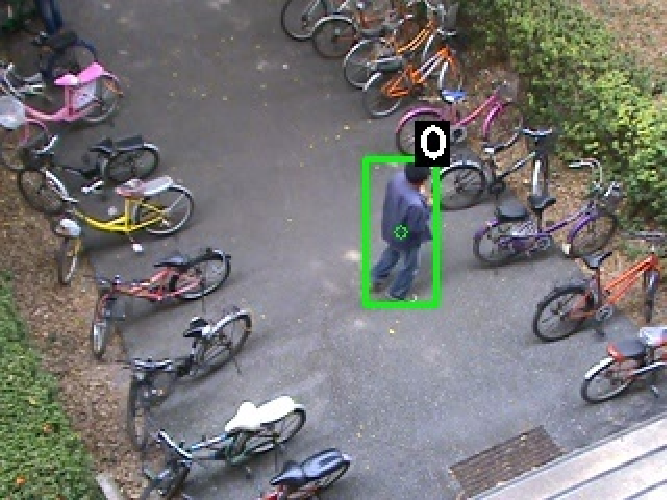
\includegraphics[scale=0.17]{figures/case-1-suspicious-0225} &
            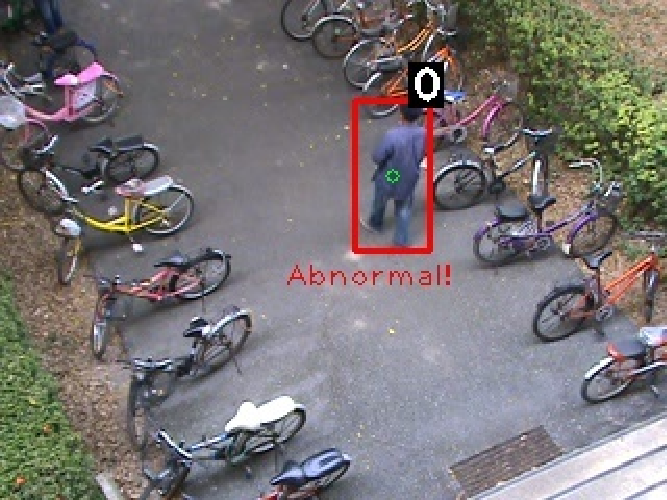
\includegraphics[scale=0.17]{figures/case-1-suspicious-0249} &
            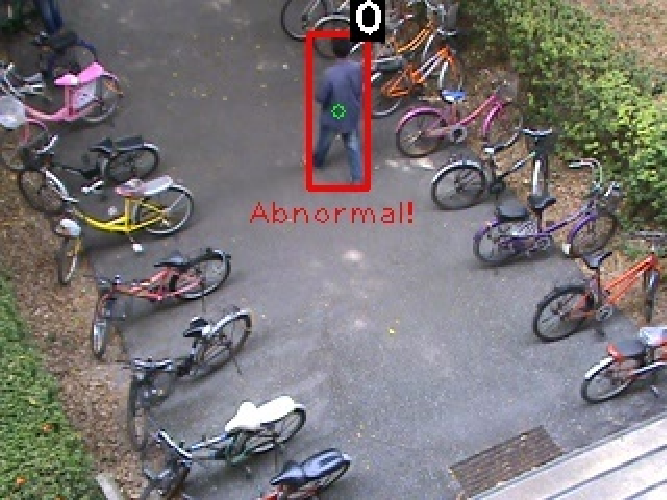
\includegraphics[scale=0.17]{figures/case-1-suspicious-0267} \\
            \small Frame 187 & 
            \small Frame 208 & 
            \small Frame 225 & 
            \small Frame 249 & 
            \small Frame 267 \\
            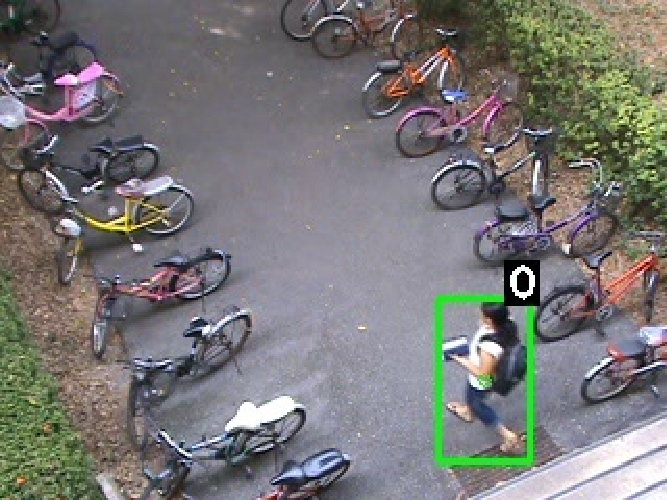
\includegraphics[scale=0.17]{figures/case-2-suspicious-0188} &
            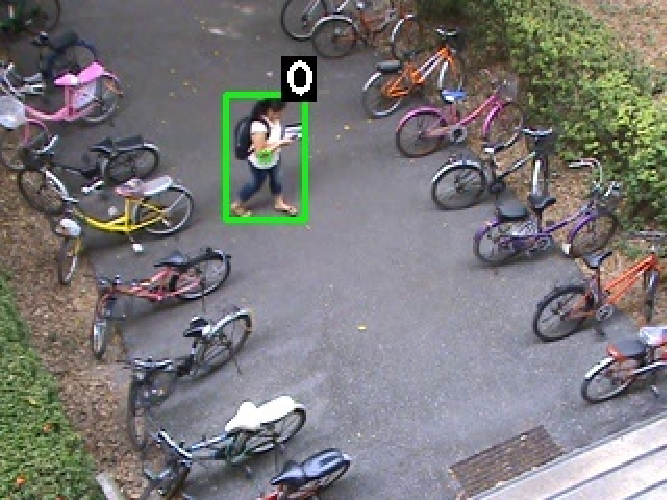
\includegraphics[scale=0.17]{figures/case-2-suspicious-0334} &
            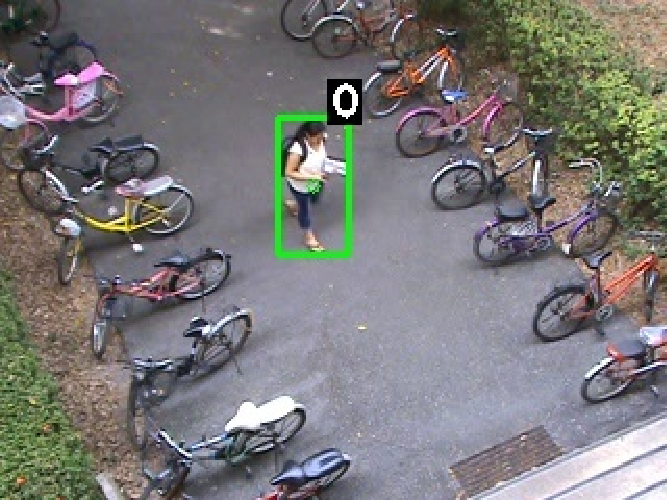
\includegraphics[scale=0.17]{figures/case-2-suspicious-0344} &
            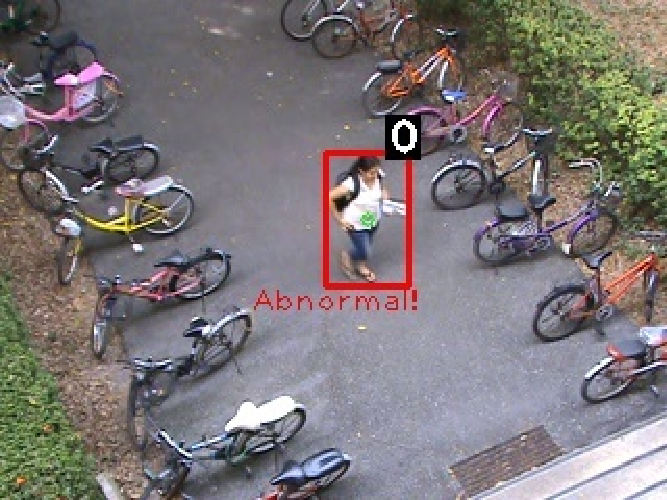
\includegraphics[scale=0.17]{figures/case-2-suspicious-0353} &
            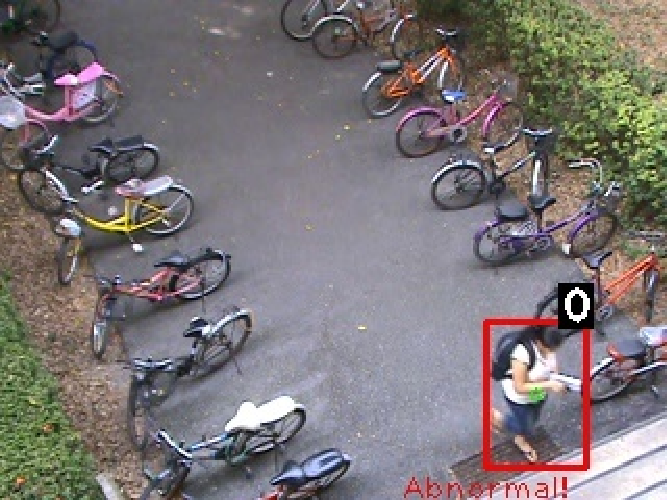
\includegraphics[scale=0.17]{figures/case-2-suspicious-0377} \\
            \small Frame 188 & 
            \small Frame 334 & 
            \small Frame 344 & 
            \small Frame 353 & 
            \small Frame 377 \\
            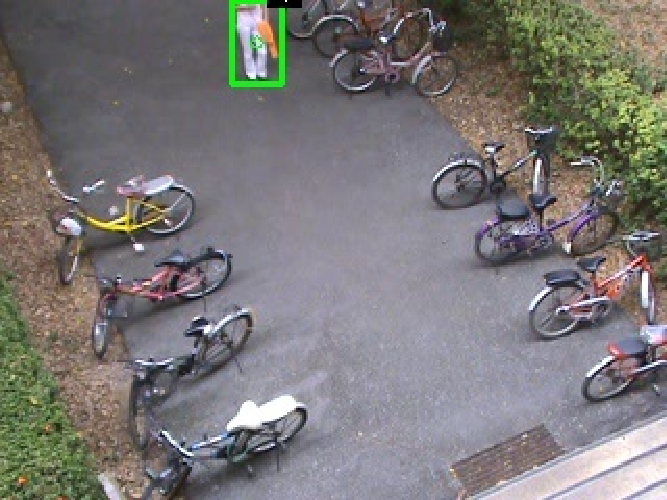
\includegraphics[scale=0.17]{figures/case-3-suspicious-0173} &
            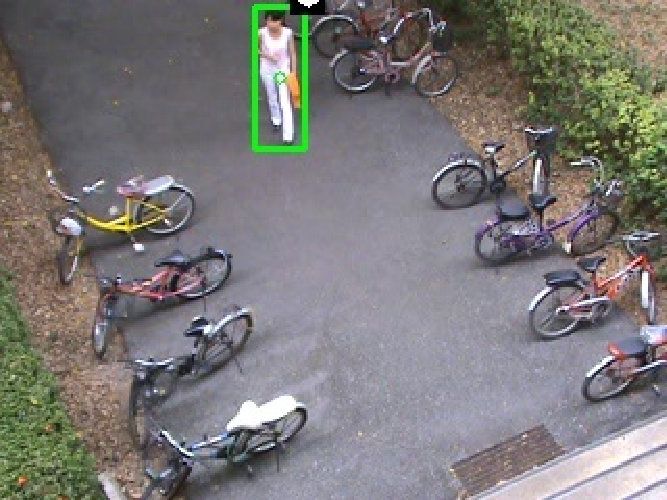
\includegraphics[scale=0.17]{figures/case-3-suspicious-0197} &
            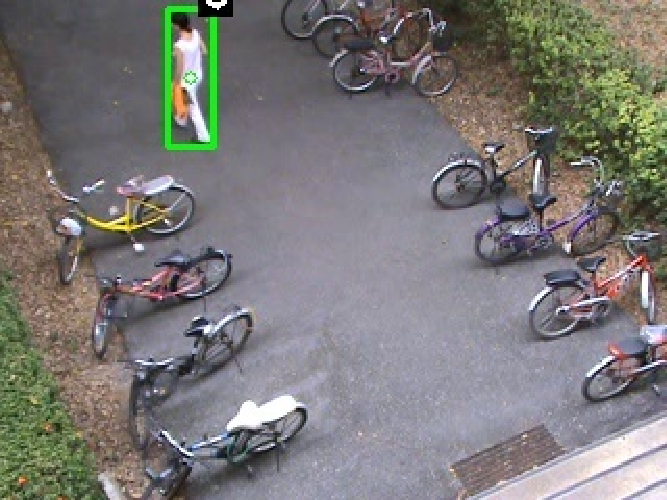
\includegraphics[scale=0.17]{figures/case-3-suspicious-0233} &
            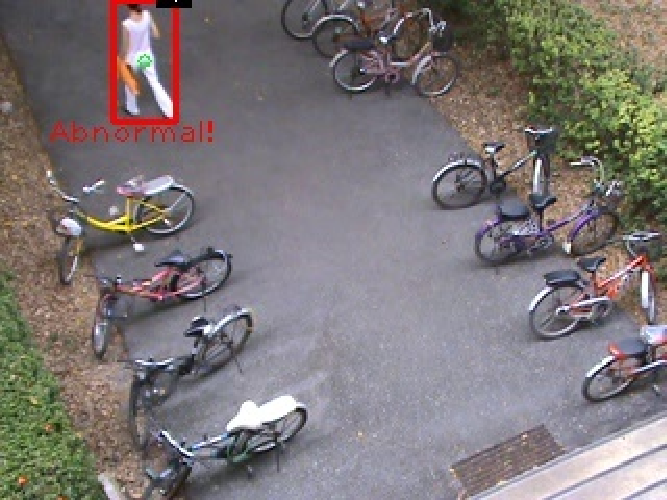
\includegraphics[scale=0.17]{figures/case-3-suspicious-0246} &
            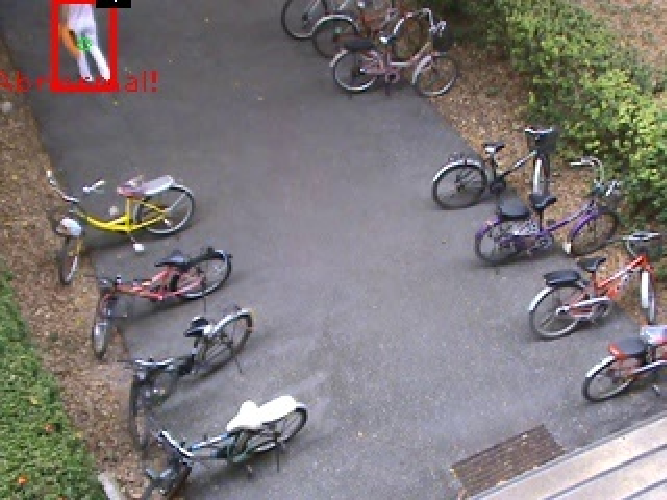
\includegraphics[scale=0.17]{figures/case-3-suspicious-0268} \\
            \small Frame 173 & 
            \small Frame 197 & 
            \small Frame 233 & 
            \small Frame 246 & 
            \small Frame 268
        \end{tabular}
        \caption{Example anomaly detected by the proposed method.}
        \label{fig:suspicious-behavior-detected}
    \end{figure}

\end{frame}

%--------------------------------------------------------------------

\begin{frame}
    \frametitle{Detection from a Small Bootstrap Set}
    \framesubtitle{Discussion}

    We have proposed and evaluated a new method for bootstrapping 
    scene-specific anomalous human behavior detection systems. 
    
    \bigskip
    
    The method requires minimal involvement of a human operator; the 
    only required action is to label the patterns in a small bootstrap 
    set as normal or anomalous. 

    \bigskip

    The experiments demonstrate that with a collection of simple HMMs, 
    it is possible to learn a complex set of varied behaviors occurring in 
    a specific scene. 

\end{frame}

%--------------------------------------------------------------------

\else

\begin{frame}
    \frametitle{Detection from a Small Bootstrap Set}
    \framesubtitle{Conclusion and Discussion}

    We have proposed and evaluated a new method for bootstrapping 
    scene-specific anomalous human behavior detection systems. 
    
    \bigskip
    
    The method requires minimal involvement of a human operator; the 
    only required action is to label the patterns in a small bootstrap 
    set as normal or anomalous. 

    \bigskip

    The experiments demonstrate that with a collection of simple HMMs, 
    it is possible to learn a complex set of varied behaviors occurring 
    in a specific scene. 

\end{frame}

%--------------------------------------------------------------------

\begin{frame}
    \frametitle{Detection from a Small Bootstrap Set}
    \framesubtitle{Pseudocode for Anomaly Detection}

    \begin{algorithm}[H]
        \caption{Anomaly Detection}
        \begin{algorithmic}
            \REQUIRE $\vec{O}$: behavior sequence
            \REQUIRE ${\cal M}$: set of HMMs
            \STATE ${\cal M}_{ab} \gets \{ M \mid M \in {\cal M} \text{~and $M$ is marked abnormal} \}$
            \STATE $( M_{ml}, L_{ml} ) \gets \textsc{Find-Most-Likely-Model}(\vec{O}, {\cal M})$
            \IF{$M_{ml} \in {\cal M}_{ab}$ or $L_{ml} \leq \theta_z$}
                \STATE $\textsc{Alert-Security-Personnel}(\vec{O})$
            \ENDIF
        \end{algorithmic}
    \end{algorithm}

\end{frame}

\fi


